\section{Worksheet 2}

\subsection{Ray Tracing}
We modify the function PointLight::Sample in order to implement hard shadows.
\begin{lstlisting}
bool PointLight::sample(const float3& pos, float3& dir, float3& L) const
{		
	dir = light_pos - pos;
	float dir_norm = length(dir);
	dir = normalize(dir);
	
	//Worksheet2 - point 1
	float epsilon = 1e-4;
	float cutoff_distance = dir_norm-epsilon;
	
	Ray shadow_ray = Ray(pos,dir,0,epsilon, RT_DEFAULT_MAX);
	HitInfo hit_info = HitInfo();
	
	tracer->trace_to_any(shadow_ray, hit_info);
	if (!hit_info.has_hit) {
		L = intensity / (dir_norm*dir_norm);
		
	}
	return !hit_info.has_hit;
}
\end{lstlisting}
\begin{figure}[H]
	\centering
	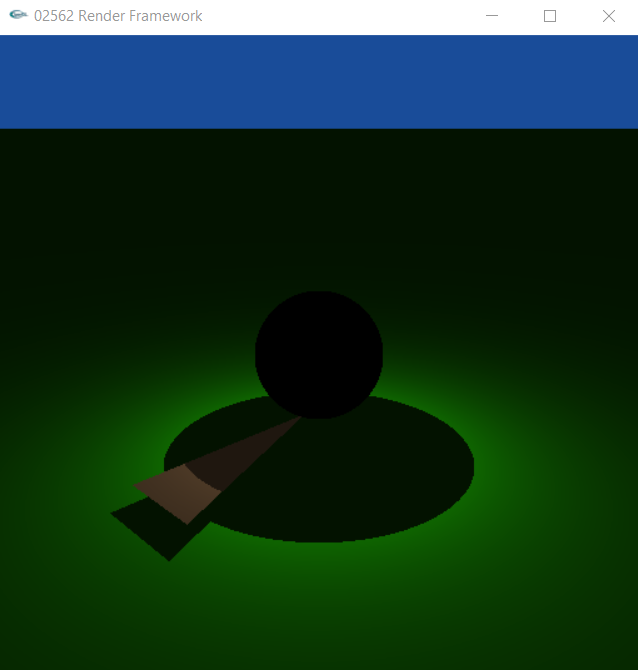
\includegraphics[scale=\imagescale]{images/worksheet_2/part_1}
	\caption{Hard shadows}
	\label{fig:hard_shadows}
\end{figure}
We want to render our sphere with a glossy material which is a mixture of between a transparent and mirror-like material. To do that we have to implement first both the shading of mirror-like and transparent materials.\\
we start first with mirror shading.
\begin{lstlisting}
bool RayTracer::trace_reflected(const Ray& in, const HitInfo& in_hit, Ray& out, HitInfo& out_hit) const
{
	float3 out_direction=reflect(in.direction, in_hit.shading_normal);
	out = Ray(in_hit.position, out_direction,0,1e-4, RT_DEFAULT_MAX);
	trace_to_closest(out, out_hit);
	float3 normal;
	out_hit.ray_ior = in_hit.ray_ior;
	out_hit.trace_depth = in_hit.trace_depth + 1;
	return out_hit.has_hit;
}

float3 Glossy::shade(const Ray& r, HitInfo& hit, bool emit) const
{
	Mirror::shade(r, hit, emit);
}
\end{lstlisting}
Then we can move to transparent shading.
\begin{figure}[H]
	\centering
	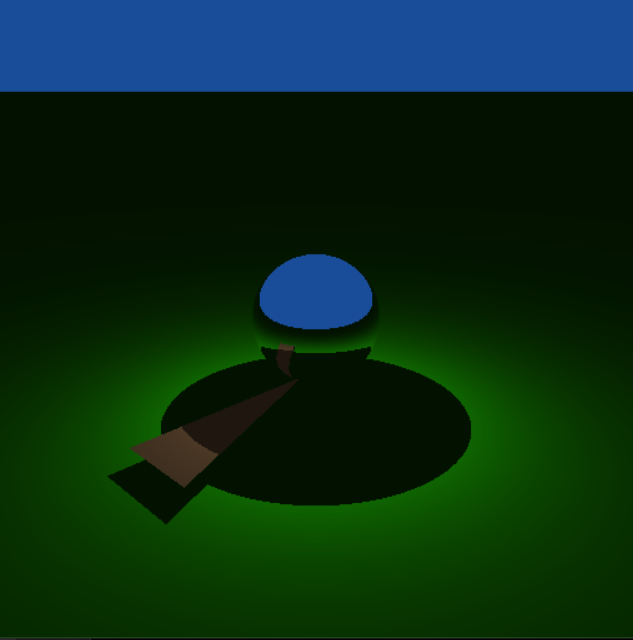
\includegraphics[scale=\imagescale]{images/worksheet_2/part_2}
	\caption{Mirror Reflections}
	\label{fig:mirror_reflections}
\end{figure}

\begin{lstlisting}
bool RayTracer::trace_refracted(const Ray& in, const HitInfo& in_hit, Ray& out, HitInfo& out_hit) const
{
	float3 normal;
	float out_ior = get_ior_out(in,in_hit,normal);
	out_hit.ray_ior = out_ior;
	bool refraction=refract(out.direction, in.direction, normal, out_hit.ray_ior / in_hit.ray_ior);
	if (refraction) {
		out.origin = in_hit.position;
		out.tmin = 1e-4;
		out.tmax = RT_DEFAULT_MAX;
		out_hit.trace_depth = in_hit.trace_depth + 1;
		
		trace_to_closest(out, out_hit);
		return out_hit.has_hit;
	}
	return refraction;
}

float3 Glossy::shade(const Ray& r, HitInfo& hit, bool emit) const
{
	Transparent::shade(r, hit, emit);
}
\end{lstlisting}
The function RayTracer::get\_ior\_out takes checks if the ray given in input hits an object, if it does then it returns the index of refraction of such material otherwise returns the index of refraction of the air which is 1.
\begin{figure}[H]
	\centering
	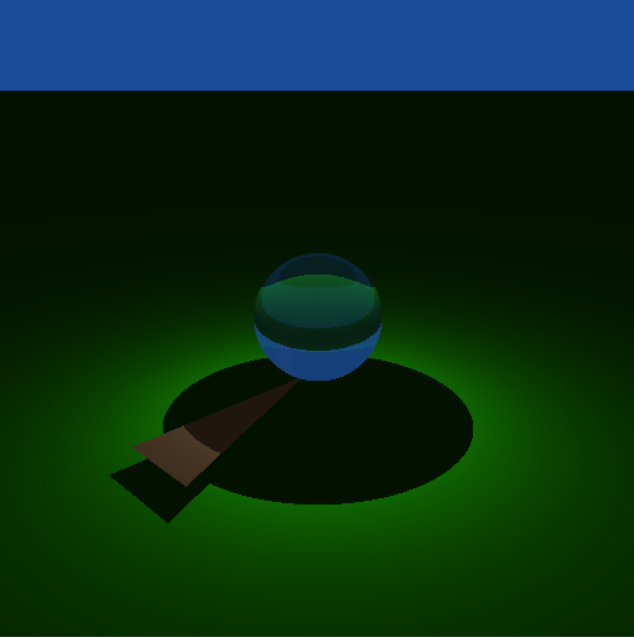
\includegraphics[scale=\imagescale]{images/worksheet_2/part_3}
	\caption{Transparent Reflections}
	\label{fig:transparent_reflections}
\end{figure}

\subsection{Phong shading}
\begin{lstlisting}
float3 Phong::shade(const Ray& r, HitInfo& hit, bool emit) const
{
	float3 rho_d = get_diffuse(hit);
	float3 rho_s = get_specular(hit);
	float s = get_shininess(hit);
	float3 radiance = make_float3(0.0f);
	
	float3 wo=-r.direction;
	for (int i = 0; i < lights.size(); i++) {
		float3 wi;
		float3 L;
		bool shade = lights[i]->sample(hit.position, wi, L);
		float3 wr=reflect(wi, hit.shading_normal);
		if (dot(wi, hit.shading_normal) > 0) {
			float3 a = rho_d/M_PIf;
			float3 b = rho_s*(s+2)/(2*M_PIf);
			float c = pow(dot(wo,wr), s);
			float3 d = a + b * c;
			float3 e = L * dot(wi, hit.shading_normal);
			radiance = radiance+d * e;
		}
	}
	return radiance;
}

float3 Glossy::shade(const Ray& r, HitInfo& hit, bool emit) const
{
	Phong::shade(r, hit, emit);
}
\end{lstlisting}

\begin{figure}[H]
	\centering
	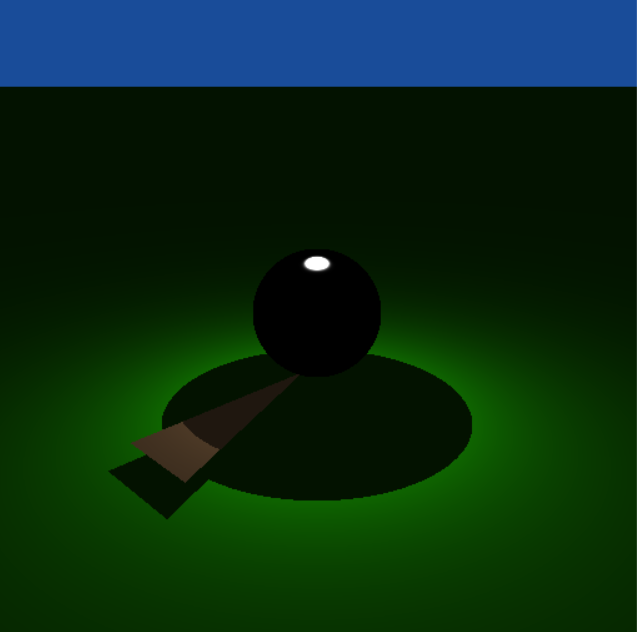
\includegraphics[scale=\imagescale]{images/worksheet_2/part_4}
	\caption{Phong illumination}
	\label{fig:phong_reflections}
\end{figure}
Our final Glossy shader renders a material which is 90\% transparent an 10\% reflective. We add also the result return by the phong reflection model to emulate the reflection of light sources.
\begin{lstlisting}
float3 Glossy::shade(const Ray& r, HitInfo& hit, bool emit) const
{
	return 0.9*Transparent::shade(r, hit, emit)+0.1*Mirror::shade(r, hit, emit)+Phong::shade(r, hit, emit);
}
\end{lstlisting}

\begin{figure}[H]
\centering
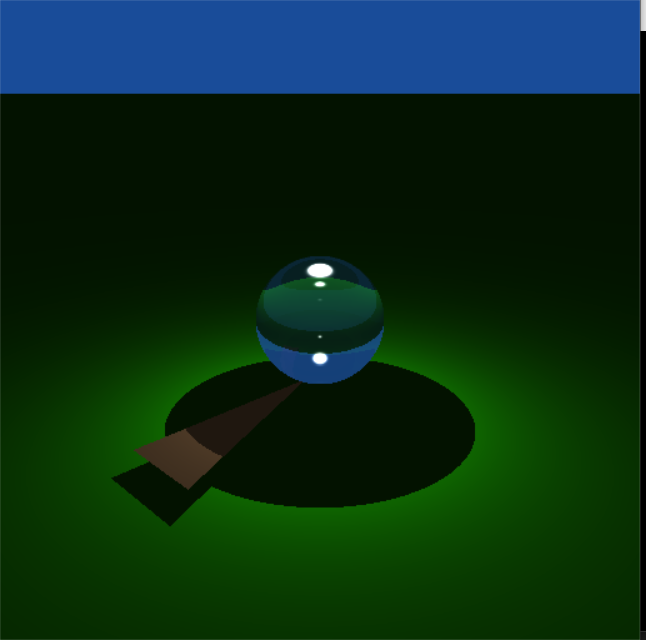
\includegraphics[scale=\imagescale]{images/worksheet_2/part_5}
\caption{Glossy illumination}
\label{fig:glossy_reflections}
\end{figure}